% =====================================================================
% Clearing-tier methodology write-ups — aligned with the committed model
% (physical IM escrow; client-clearing solvency CFTC Reg 1.17 cash/IM>=8% for BOTH tiers, plus a
%  bank-only Basel/eSLR leverage ratio cash/exposure>=4.25% deleverage trigger for BCMs (NBCM $0.5-3B,
%  client 4% freeze); 2x own-book cap; 15% client house margin; FHS close-to-close IM (q99=3.0, ~11d EWMA);
%  liquidity default; member CCP transfer-at-0.80 reassigned to the largest-opposing survivor
%  (inventory/cash-conserving); EMIR-48 porting; cover-2 SLOIM fund; 5-level waterfall, IM seized first).
%
% Destinations: §A participants (agents section); §B margin & the funding
% cycle (margin-call section, right after the agents); §C default management.
% Citation keys follow references.bib (cftc_fcm, haynes_mcphail_zhu_2019,
% acosta_smith_2018, thurner_2012, aymanns_farmer_2015, basel_frtb, emir_rts,
% simudyne_odd, almgren_chriss_2000, vuillemey_2020, euronext_a9).
% =====================================================================


% ============== §A — PARTICIPANTS (agents section) ===================

\paragraph{Banking clearing member (BCM).}
There are ten BCMs. All ten trade a proprietary (house) account through the fundamental-trader
logic of Section~\ref{sec:agents}, so for the market-layer calibration the thirty fundamental
traders and ten BCMs form a single forty-strong fundamental-equivalent population and the
calibration is unaffected by the clearing cast; five of the ten additionally provide
client-clearing services. Each BCM carries bank-FCM-scale loss-absorbing capital drawn from
$U[\$5,\$10]$\,billion \citep{cftc_fcm}. Its solvency is governed by a \emph{leverage ratio} ---
unencumbered capital over cleared exposure,
\begin{equation}
\label{eq:kappa}
\kappa_\tau \;=\; \frac{C_\tau}{E_\tau} \;\ge\; 4.25\%,
\qquad
E_\tau \;=\; \bigl(|N^{\mathrm{own}}_\tau| + \textstyle\sum_c |N^{c}_\tau|\bigr)\,\ell\,\chi\,m_\tau,
\end{equation}
where $C_\tau$ is cash net of posted initial margin and $E_\tau$ is the USD notional of the
member's own book and its cleared-client book. The $4.25\%$ floor is the Basel III / US-eSLR
leverage ratio for a global systemically important bank --- the $3\%$ base plus the
surcharge-linked buffer --- rather than a margin-coverage ratio, the constraint that actually binds
for derivative dealers \citep{haynes_mcphail_zhu_2019,acosta_smith_2018}, and the channel through which
leverage-constrained intermediaries propagate stress \citep{thurner_2012,aymanns_farmer_2015}.
Because initial margin is escrowed at the CCP (Section~\ref{sec:margin}), a rising margin in stress
lowers $C_\tau$ and tightens $\kappa$ through the numerator --- a funding-liquidity squeeze that
compounds the effect of an enlarging book. A banking member is, in addition, held to the same FCM
client-clearing rule as the non-banks --- CFTC Reg.~1.17, $C_\tau/\mathrm{IM}_\tau \ge 8\%$ on its
client book (the solvency measure common to both tiers, Section~\ref{sec:default}), so the two member
types are compared on the same client-clearing yardstick. The bank leverage ratio
\eqref{eq:kappa} is the additional, binding constraint that triggers the own-book deleverage below;
a non-bank, holding no own account, is not subject to it.

The proprietary book is additionally bounded by a static gross-leverage limit,
$|N^{\mathrm{own}}_\tau| \le 2\,C_\tau$ --- a flat position cap with no volatility input, in the
spirit of a trading-book risk limit \citep{basel_frtb}. It is deliberately modest: a realistic
dealer proprietary book that is a minority of the member's much larger client-clearing book, so the
house share of posted margin remains a minority (consistent with the empirical $\sim$18\% house /
$\sim$82\% client split of cleared margin). The member's leverage ratio is therefore driven by its
\emph{client} book: in the stressed regime the variation-margin losses on the cleared-client
positions, compounded by the procyclical rise in escrowed margin, push $\kappa$ below the floor,
while in the calm regime it stays comfortably above it --- so the corrective response activates only
under stress, and through the client-clearing channel rather than a self-inflicted proprietary
blow-up.

On breaching the $4.25\%$ floor a BCM takes regulatory corrective action: it \emph{deleverages} its
own book over an Almgren--Chriss schedule \citep{almgren_chriss_2000} toward a $6\%$ buffer above
the floor (so it does not immediately re-breach on the next mark), and simultaneously
\emph{freezes} --- submitting no new own-account risk and admitting no new client risk --- until
its ratio recovers. Reducing exposure below the leverage minimum is the Basel/CFTC requirement, and
the resulting open-market sales are the forced-deleveraging contagion channel
\citep{thurner_2012,aymanns_farmer_2015}. Only the own book can be shed intraday, so a member whose
exposure is dominated by its client book sheds all of its own risk and then freezes on the
residual. Liquidation of the member's \emph{entire} book occurs only on outright default
(Section~\ref{sec:default}).

\paragraph{Non-banking clearing member (NBCM).}
There are five NBCMs --- pure clearing intermediaries that hold no proprietary position and submit
no orders to the book, so their only exposure is the client book they carry. Each carries
non-bank-FCM-scale capital, $U[\$0.5,\$3]$\,billion \citep{cftc_fcm} --- the substantial non-bank
clearers (Marex, ABN~AMRO Clearing, Clear~Street) that carry real client volume. A non-bank is not
subject to the Basel leverage ratio; it is governed instead by the \textbf{CFTC Reg.~1.17}
net-capital rule --- adjusted net capital at least $8\%$ of risk maintenance margin, i.e.\
$C_\tau/\mathrm{IM}_\tau \ge 8\%$ on its client book. Holding no own account, an NBCM posts no own
margin and is reached by the margin cycle only through its clients --- it is squeezed when they are,
and absorbs any client shortfall it must cover. On breaching the floor it has no proprietary book to
shed and therefore simply \emph{stops out} (a liquidity defaulter, as at Nasdaq~2018 and the
LME~2022), preserving the reference model's BCM-deleverage / NBCM-stop asymmetry \citep{simudyne_odd}. The
distinction between a BCM and an NBCM is thus both structural --- capital scale, the presence of a
proprietary book, and loss priority in the waterfall --- and behavioural at the floor (deleverage
versus stop-out).

\paragraph{Clients.}
Clients are leveraged end-users that clear through a member (the tiered baseline) or, in the H1
counterfactual, face the CCP directly. Clients are assigned to members by a capacity-proportional
(leverage-balanced) rule --- each client is routed to the member whose resulting client-book-to-capital
ratio would be lowest --- so the largest asset-manager books clear through the highest-capital
bank-members and the smaller accounts through the non-bank members, the realistic ordering, which
leaves every member at a comparable gross leverage. Each client carries its own balance sheet --- cash, a net
futures position, the initial margin it has posted to the CCP through its member, and its cumulative
variation margin. Its initial capital is set to its institutional scale, a fraction of the
bank-scale members it clears through: asset-manager (fundamental) clients are drawn from
$U[\$0.5,\$3]$\,billion, CTA / trend-following (momentum) clients from $U[\$0.2,\$1]$\,billion,
and noise (zero-intelligence) accounts from $U[\$0.2,\$0.5]$\,billion. A client may open a position
only up to its broker \emph{house margin}: a fixed $15\%$ of notional, i.e.\ $\approx$6.67-times
leverage. That figure is the post-2020 statutory minimum customer margin
for security futures (CFTC/SEC, 17~CFR~242.400--406 and 41.42--49 --- $20\%$ of current value from
2002, lowered to $15\%$ in 2020) \citep{cftc_sec_secfutures_margin}, used here as the
house margin: it sits well above the $\sim$5--7\% SPAN minimum the exchange itself charges on the
index future, reflecting the add-on an FCM imposes on a leveraged client --- FCMs may, and do,
require margin above the exchange floor \citep{nfa_margins}. Each margin cycle a client settles
variation margin in cash and posts its own (procyclical) initial margin through its member to the
CCP (Section~\ref{sec:margin}); it is additionally frozen by its FCM near distress (cash over
exposure $\le 4\%$). A client that cannot meet a variation- or
initial-margin call from its own cash defaults. On a client default its member assumes the position
and closes it out in the open market over an Almgren--Chriss schedule \citep{almgren_chriss_2000};
the client's posted margin is first-loss and the member bears the residual --- the first link in the
contagion chain.


% ============== §B — MARGIN AND THE FUNDING CYCLE (margin-call section) ===========

\paragraph{Initial margin.}
The CCP charges initial margin on a participant's \emph{gross} exposure --- a member's own book plus
the gross notional of its client book, $\sum_c |N^c_\tau|$ (the absolute client positions summed, with
no netting of one client's longs against another's shorts). The margin rate is a $99\%$ price move over
the close-out horizon, floored at an anti-procyclicality minimum \citep{emir_rts}:
\begin{equation}
\label{eq:im}
f_\tau = \max\!\bigl(6\%,\;\; \alpha_{99}\,\sigma^{\mathrm{daily}}_\tau\,\sqrt{\mathrm{MPOR}}\,\bigr),
\qquad \alpha_{99} = 3.0,\quad \mathrm{MPOR} = 2\ \text{days},
\qquad \mathrm{IM}_\tau = f_\tau \times \text{exposure}.
\end{equation}
Reading the rate left to right: $\sigma^{\mathrm{daily}}_\tau$ is the daily \emph{close-to-close}
return volatility --- an exponentially-weighted average of recent returns ($\sim$11-day half-life, the
RiskMetrics $\lambda\approx0.94$ convention) that adds the overnight-gap variance to the intraday
variance, so the margin covers the between-session jump it is marked across (in the stressed window
$\sim$45\% of daily variance is overnight); $\sqrt{\mathrm{MPOR}}$ scales that one-day move up to the two-day
close-out window, because volatility grows with the square root of time; and $\alpha_{99}=3.0$ is the
$99\%$ quantile of volatility-standardised E-mini S\&P~500 returns, taken \emph{empirically} ---
filtered historical simulation, the standard CCP method --- rather than from a normal curve, because
index futures are fat-tailed and the Gaussian quantile ($2.33$) understates the true $99\%$ move by
about a third. The $6\%$ floor is the anti-procyclicality minimum (EMIR Art.~28): in quiet markets the
raw VaR sits below it, so margin holds at $6\%$; in stress the VaR term takes over and the rate climbs
with volatility (to $\sim$12--25\%). Initial margin is \emph{recalculated every (hourly) margin
cycle}: the volatility estimate is refreshed on the latest returns, the rate $f_\tau$ is recomputed,
and each participant's escrowed margin is trued up to $f_\tau \times$ its current exposure --- extra
cash is called in when the rate or the position has risen (the procyclical funding drain in a stress
spike) and margin is released back as they fall. This reactive recomputation is the baseline; the
\emph{flat} and \emph{static} regimes instead hold the rate fixed, as comparators for the
procyclicality hypothesis. A cleared client posts its \emph{own} initial margin: the CCP's call passes
down through its clearing member, the client funds it from its own cash, and the member transfers it to
the CCP --- a pass-through that leaves the member holding none of the client's market risk unless that
client defaults.

\paragraph{Variation margin.}
Variation margin is settled on a fixed hourly cycle, \emph{unconditionally}: each cycle every position
is re-marked to the current price and its \emph{full} profit or loss is moved in cash to or from the
holder's account that same cycle --- a paper move becomes an immediate cash flow, never an accruing
unmargined loss. Because the initial margin is also re-posted each cycle (above), a participant is
always collateralised to the full IM; the $95\%$-of-IM maintenance level only \emph{flags} a cycle
whose move exceeds $5\%$ of posted IM --- a margin-call-sized shock --- for monitoring, and does not
gate the settlement. A future carries no principal, so a trade moves only the position; cash changes
hands only through this cycle, and posted initial margin sits as cash in the CCP's segregated account,
returned as the position closes and seized first if the holder defaults. A participant whose own cash
is exhausted by a variation-margin call --- or that cannot fund the re-posted initial margin ---
\emph{defaults}, making default a funding (liquidity) event, the way clearing members actually fail
(Nasdaq~2018, LME~2022).


% ============== §C — DEFAULT MANAGEMENT (default-management section) =============

\paragraph{Close-out.}
The two tiers resolve a default differently. A defaulted \emph{client} is closed out by its own
\emph{member}, which assumes the position and liquidates it on the open market over an Almgren--Chriss
schedule \citep{almgren_chriss_2000}: a single client's book is small enough for open-market execution
to be realistic, and the resulting book-walk is the client-level price-impact channel. A defaulted
\emph{member} (or, in the direct-clearing counterfactual, a direct client) is resolved by the
\emph{CCP}: its posted initial margin is seized first --- the defaulter's own first-loss resource
(EMIR Art.~45(1)) --- and the residual book is \emph{transferred} to the surviving member with the
largest opposing position (the natural auction winner) at a recovery rate of $0.80$, the $20\%$
haircut passing into the waterfall. Reassigning the book rather than writing it off conserves system
positions and cash through the cascade. The $0.80$ recovery sits between a liquid, hedged book closed
out within its own margin (Lehman/LCH 2008) and a concentrated, illiquid one that exhausts it and
draws the mutualised fund (Nasdaq/Aas 2018) \citep{bell_holden_2018,vuillemey_2020}; two off-baseline
stress arms sharpen the channel --- an open-market CCP disposal (loss endogenous to crash liquidity,
with its own price impact) and a disorderly $0.60$ recovery. Any open liquidation is completed by
session end, so no assumed book crosses the overnight gap.

\paragraph{Porting.}
On a member default the CCP first tries to \emph{port} the defaulter's surviving clients to other
client-clearing members that retain capital headroom after taking them on (EMIR Art.~48). Porting is
capacity-checked: clients that cannot be placed are closed out and frozen flat --- reproducing the
fragility of client porting under stress, where a cleared client typically depends on a single
clearing agent.

\paragraph{Default fund.}
Whatever loss survives the defaulter's own margin is met by a cash-prefunded, mutualised default
fund, sized \emph{cover-2}: large enough for the two most-exposed members to fail together. Each
member's \emph{stress shortfall} --- its loss beyond its own margin in an extreme move --- is
\begin{equation}
\label{eq:sloim}
L_i = \max\!\bigl(0,\; (s - f)\,E_i\bigr),
\end{equation}
with $E_i$ the member's exposure, $f$ its margin rate, and $s$ an extreme-but-plausible two-day move
--- the same empirical (filtered-historical-simulation) quantile family as the IM, but at a higher
$\sim$99.9\% confidence and floored at the historical $10\%$ \citep{euronext_a9}. The fund covers the two largest
shortfalls plus a prudential buffer, and the exchange pre-funds a thin slice of it as
skin-in-the-game (consumed ahead of the mutualised member pool, but after the defaulter's own
resources; the $3\%$ below is mid-range of the levels CCPs disclose, \citealp{cpmi_iosco_pqd}):
\begin{equation}
\label{eq:df}
\mathrm{DF} = (1+b)\,\bigl(L_{(1)} + L_{(2)}\bigr), \qquad b = 10\%, \qquad
\mathrm{SITG} = 3\%\times\mathrm{DF},
\end{equation}
where $L_{(1)} \ge L_{(2)}$ are the two largest member shortfalls. Each member pre-funds its share in
cash in proportion to its margin; a non-bank member's share rests entirely on its \emph{gross} client
book.

\paragraph{The default waterfall.}
A loss that survives close-out --- the defaulter's unpaid variation margin plus the close-out haircut
--- is absorbed in a fixed order (EMIR Art.~45), shown in Figure~\ref{fig:waterfall}: the
\emph{defaulter's} own resources first (the ``defaulter-pays'' principle), then the CCP's own
first-loss slice, then the \emph{mutualised} layers shared across surviving members, and the CCP's
capital only as a last resort. The deepest layer a default reaches is the model's headline measure of
how far stress travels beyond the defaulter: in the calm and stressed (COVID) baselines it halts at
the seized margin, and the mutualised layers are reached only when a structural buffer is removed
(direct clearing) or the close-out is disorderly.

\begin{figure}[tb]
\centering
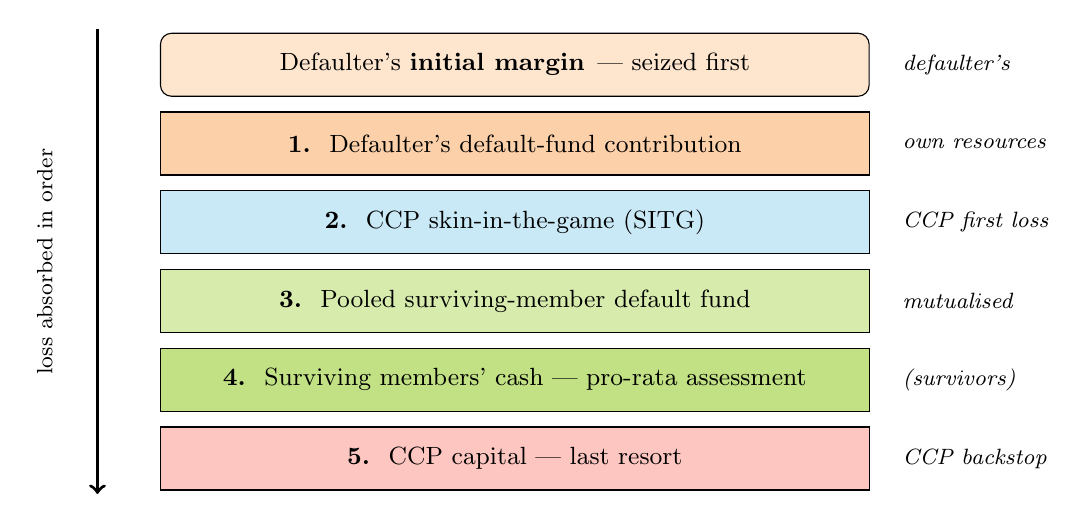
\begin{tikzpicture}[font=\small, every node/.style={align=center}]
  % tranches, top (consumed first) to bottom (consumed last)
  \node[draw, rounded corners, fill=Apricot!30,  minimum width=9cm, minimum height=0.8cm] at (0, 0) {Defaulter's \textbf{initial margin}\, --- seized first};
  \node[draw, fill=Apricot!55,    minimum width=9cm, minimum height=0.8cm] at (0,-1) {\textbf{1.}\; Defaulter's default-fund contribution};
  \node[draw, fill=SkyBlue!45,    minimum width=9cm, minimum height=0.8cm] at (0,-2) {\textbf{2.}\; CCP skin-in-the-game (SITG)};
  \node[draw, fill=YellowGreen!40,minimum width=9cm, minimum height=0.8cm] at (0,-3) {\textbf{3.}\; Pooled surviving-member default fund};
  \node[draw, fill=YellowGreen!60,minimum width=9cm, minimum height=0.8cm] at (0,-4) {\textbf{4.}\; Surviving members' cash --- pro-rata assessment};
  \node[draw, fill=Salmon!45,     minimum width=9cm, minimum height=0.8cm] at (0,-5) {\textbf{5.}\; CCP capital --- last resort};
  % consumption-order arrow
  \draw[->, very thick] (-5.3,0.45) -- (-5.3,-5.45);
  \node[rotate=90, anchor=south] at (-5.75,-2.5) {\footnotesize loss absorbed in order};
  % grouping labels
  \node[anchor=west] at (4.8, 0)   {\footnotesize\itshape defaulter's};
  \node[anchor=west] at (4.8,-1)   {\footnotesize\itshape own resources};
  \node[anchor=west] at (4.8,-2)   {\footnotesize\itshape CCP first loss};
  \node[anchor=west] at (4.8,-3)   {\footnotesize\itshape mutualised};
  \node[anchor=west] at (4.8,-4)   {\footnotesize\itshape (survivors)};
  \node[anchor=west] at (4.8,-5)   {\footnotesize\itshape CCP backstop};
\end{tikzpicture}
\caption{\textbf{The CCP default waterfall.} A default's loss is absorbed top-down. The defaulter's
own resources --- its seized initial margin, then its default-fund contribution --- absorb first; the
CCP's skin-in-the-game follows; only then is the loss mutualised across surviving members (the pooled
fund, then a pro-rata cash assessment); the CCP's own capital is the final backstop. In the baseline
regimes the cascade halts at the first tranche.}
\label{fig:waterfall}
\end{figure}
